\subsubsection{\theoryC{Precision searches in dijets at the HL-LHC and HE-LHC}}
\contributors{S. V. Chekanov, J. T. Childers, J. Proudfoot, R.Wang, D. Frizzell}
%{\bf Author(s):} S. V. Chekanov$^1$, J. T. Childers$^2$, J. Proudfoot$^3$, R.Wang$^4$, D. Frizzell$^5$
%
%\vspace{1cm}
%
%$^1$ chekanov@anl.gov,  HEP Division, Argonne National Laboratory, 9700 S.~Cass Avenue, \\ Argonne, IL 60439, USA.
%
%$^2$ jchilders@anl.gov, HEP Division, Argonne National Laboratory, 9700 S.~Cass Avenue, \\ Argonne, IL 60439, USA.
%
%$^3$ proudfoot@anl.gov, HEP Division, Argonne National Laboratory, 9700 S.~Cass Avenue, \\ Argonne, IL 60439, USA.
%
%$^4$ Rui.Wang@cern.ch, HEP Division, Argonne National Laboratory, 9700 S.~Cass Avenue, \\ Argonne, IL 60439, USA.
%
%$^5$ dylan.frizzell@ou.edu, Homer L. Dodge, Department of Physics and Astronomy, \\ University of Oklahoma, Norman, OK, USA.
%
%\vspace{1cm}

Model-independent searches for deviations in dijet invariant mass distributions ($M_{jj}$) predicted by the Standard Model is one of the central studies at the LHC.
The main goal of such searches is to find small deviations from background distributions, under the assumption that a new resonant state decaying to partons that form two jets may introduce an excess in dijet masses localized around the resonance mass.
In recent years, such searches for new physics at the LHC have been performed  by both ATLAS and CMS collaborations (see the recent studies in \citeref{Aad:2015xis,2016229, Aaboud:2017yvp, Khachatryan:2010jd, Chatrchyan:2013qha, Sirunyan:2016iap,Aaboud:2017yvp,Aaboud:2018fzt}), but no statistically significant deviations from background expectations were found. Such searches are usually performed for resonances with a width of up to 15\% of the resonance mass. Searches for broader resonances are usually more 
difficult since the available tools to determine the background 
hypothesis have a number of limitations that do not allow for 
reliable estimates of background shapes in the presence of broad resonances.  
Despite the generality of dijet searches, such studies can exclude a number of BSM models, such as models with  quantum black holes, excited quarks, and $Z'$ bosons and so on.
Currently, the LHC run II data provide the 95\%~\cl exclusion limits on BSM resonances up to 6.5~TeV in masses.

\begin{figure}[h]
\begin{center}
   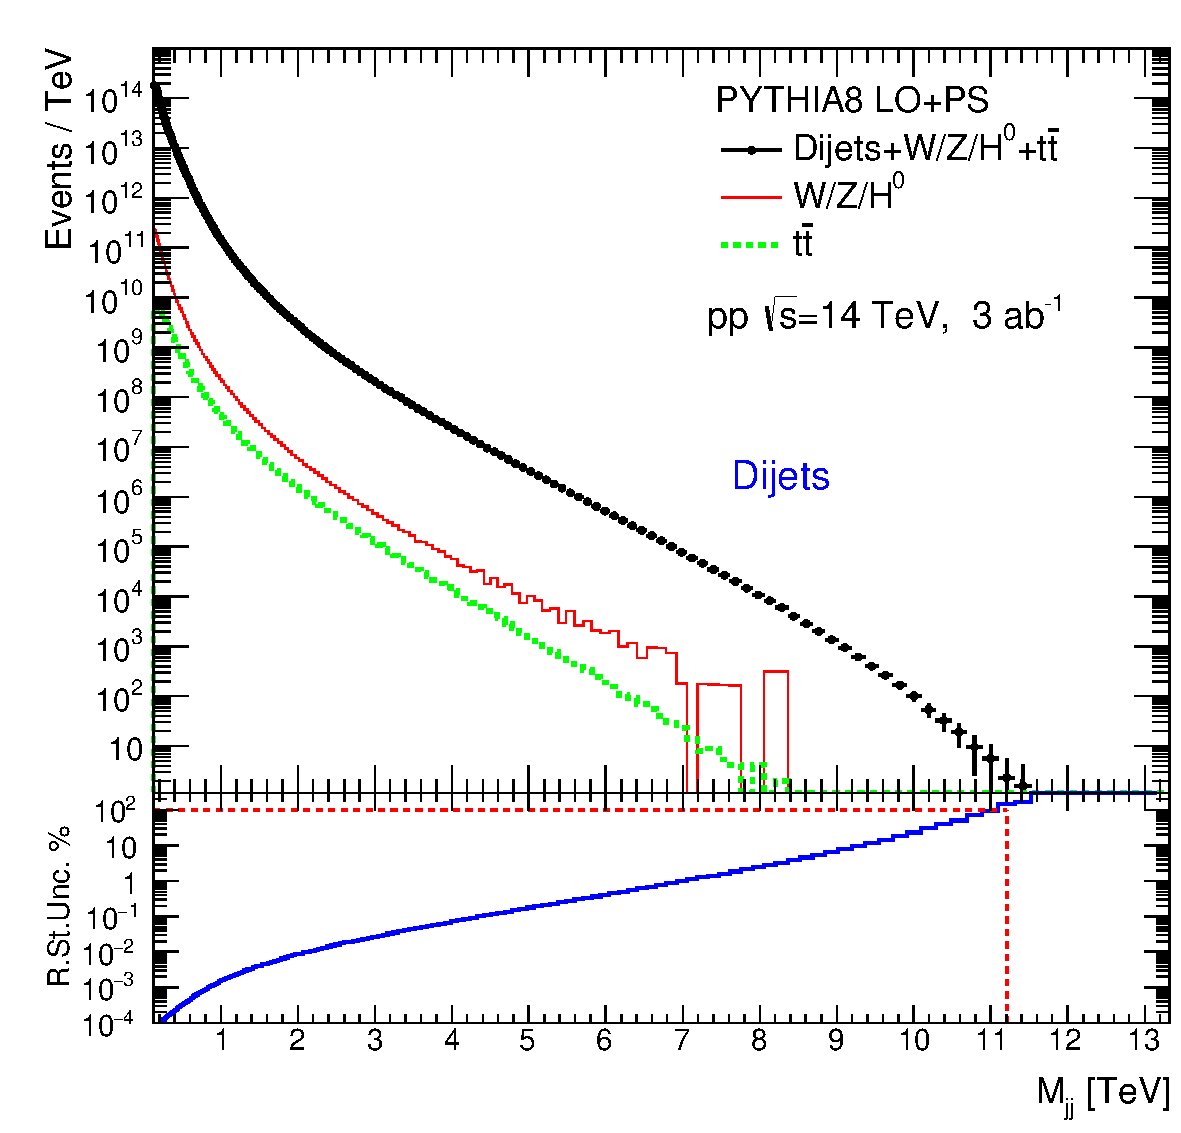
\includegraphics[width=0.45\textwidth]{\main//section7OtherSignatures/img/14tev_JetJetMass_2jet_3000fb}
   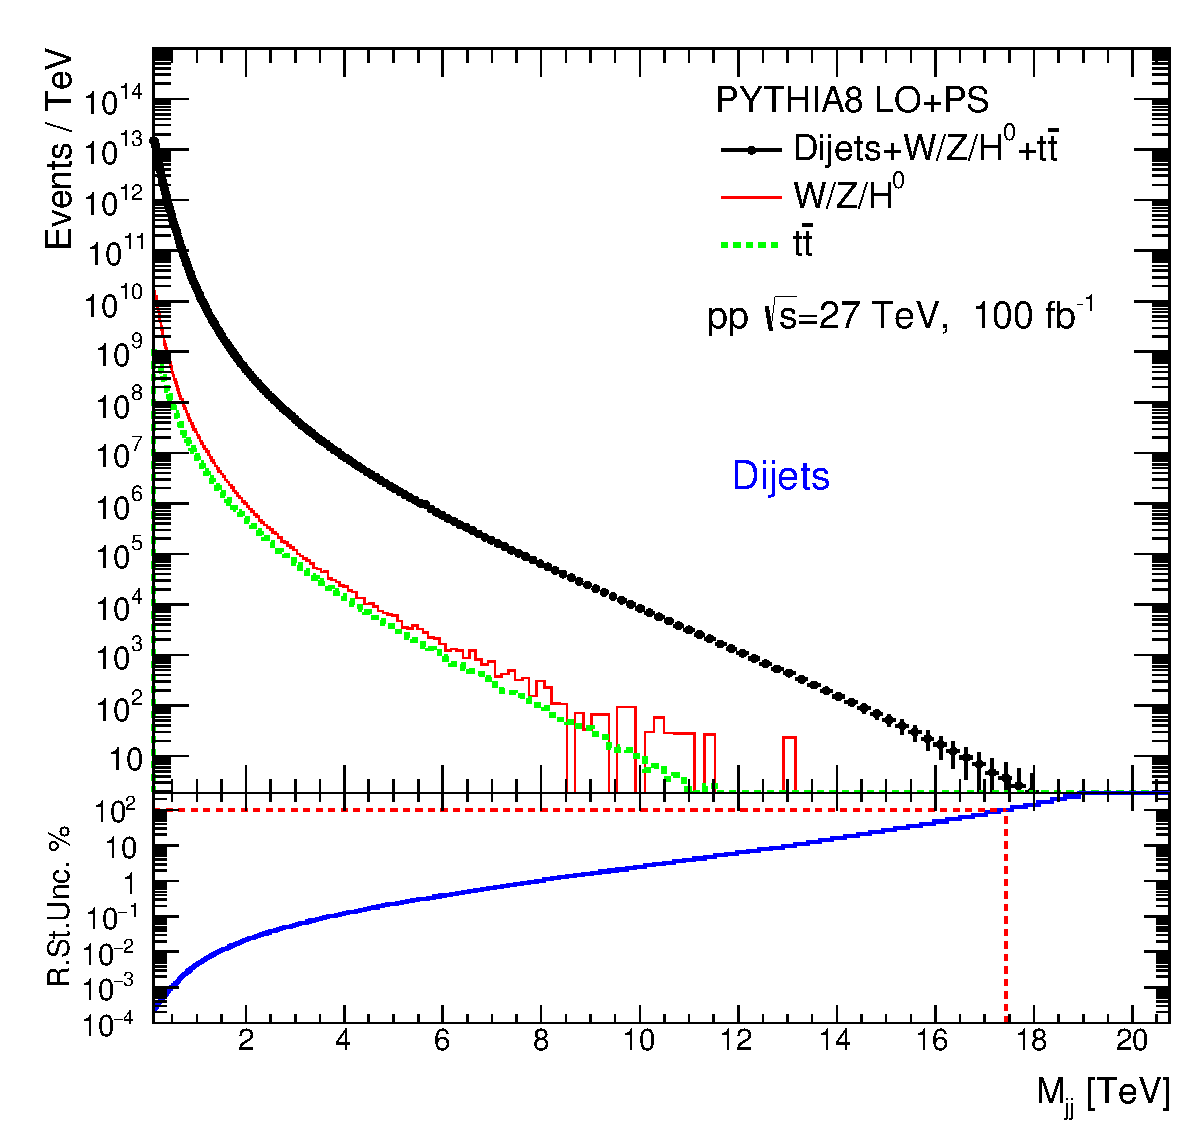
\includegraphics[width=0.45\textwidth]{\main//section7OtherSignatures/img/27tev_JetJetMass_2jet_100fb}
\end{center}
\caption{Expectations for the dijet invariant mass distribution for 3~ab$^{-1}$ at HL-LHC and
100 fb$^{-1}$ at the HE-LHC using the Pythia generator. Contributions
from  $W/Z/H^0$ -boson processes and top-quark processes are shown separately (without stacking the histograms). The bottom plots show the relative  statistical uncertainties in each bin, together with the line indicating the mass point at which the uncertainty is $100\%$. The figures are taken from~\cite{Chekanov:2017pnx}.}
\label{fig:14tev_JetJetMass_2jet}
\end{figure}

\begin{figure}[ht]
\begin{center}
   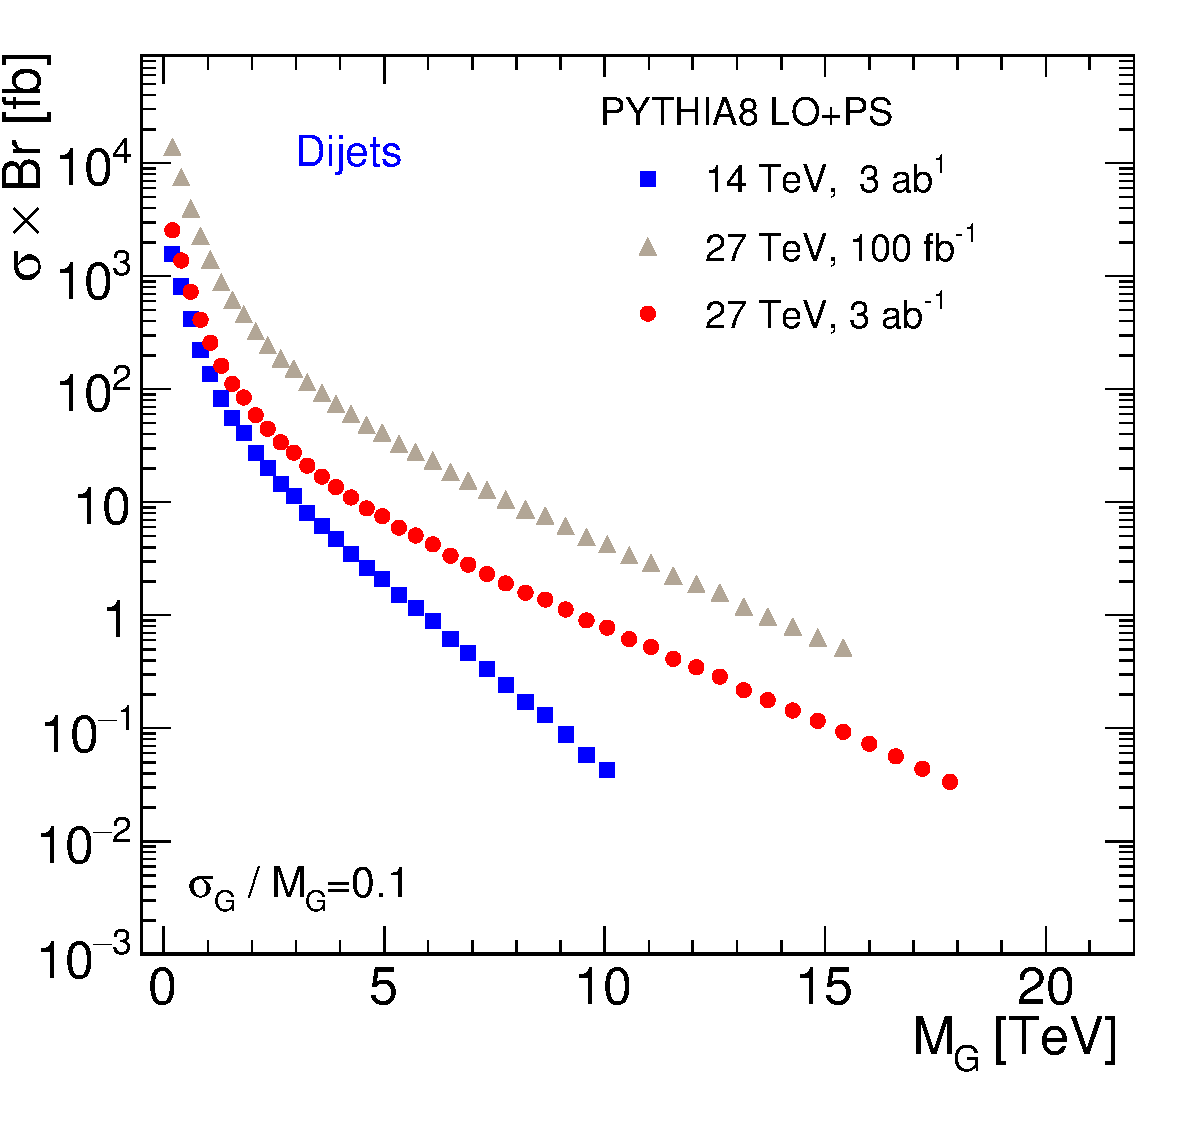
\includegraphics[width=0.45\textwidth]{\main//section7OtherSignatures/img/JetJetMass_2jet.pdf}
   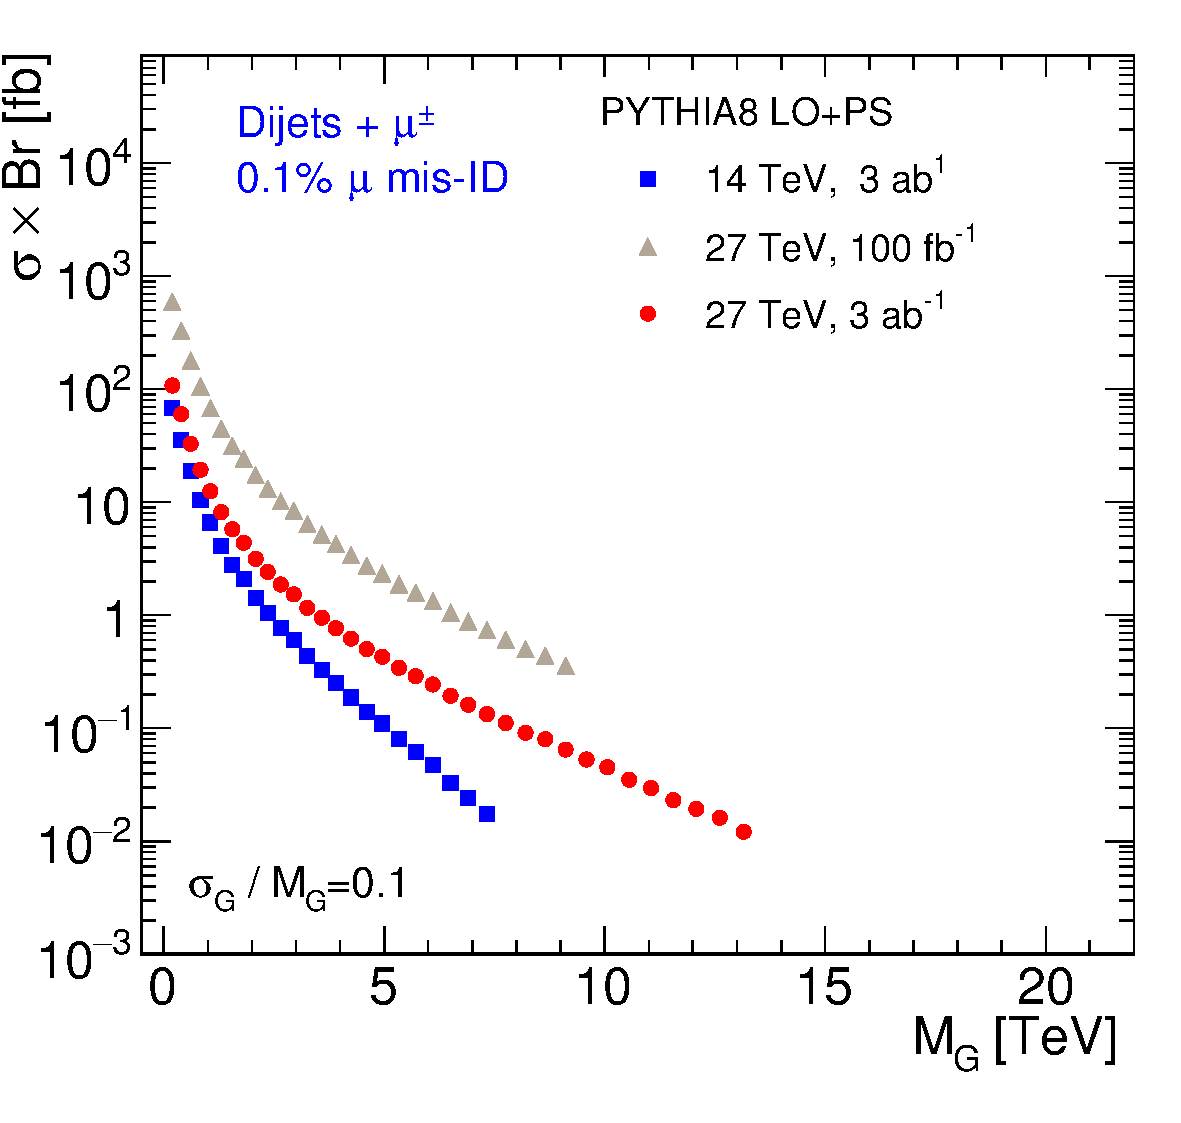
\includegraphics[width=0.45\textwidth]{\main//section7OtherSignatures/img/JetJetMass_2jet_lep_mu.pdf}
\end{center}
\caption{The 95\%~\cl upper limits obtained from the
$M_{jj}$  distribution on fiducial cross-section times the  branching ratio to two jets
for a hypothetical BSM signal approximated by a Gaussian contribution to the dijet mass spectrum.  The limits are obtained for the HL-LHC and HE-LHC energies. The figure shows the limits for inclusive dijet production (left) and for events with at least one isolated muon with $p_T>60$~GeV.}
\label{fig:JetJetMass_jet}
\end{figure}


Shapes of the background $M_{jj}$ distributions can be affected by several instrumental factors, making
such studies difficult for low-mass regions where statistics are large.
In the case of inclusive jet production, the rate of dijets is reduced  due to triggers with low acceptance rate, which leads to complicated shapes of in the region of $M_{jj}$ below 1~TeV. 
This leads to difficulties in interpretation of the shapes
of the $M_{jj}$ distributions using QCD-motivated fit functions.
Recently, such searches have been extended to less inclusive events, such as events with $b-$jets and  associated leptons~\cite{Aaboud:2018tqo,Collaboration:2320658}. These studies rely on less inclusive triggers with low thresholds, thus accessing regions with small dijet masses. 

With increase in LHC luminosity, searches for new physics beyond the Standard Model in the invariant mass of two jets become increasingly important since the large event rate allows one to explore a large $M_{jj}$ phase space with improved statistics.  The proposed HL-LHC and HE-LHC experiments will open a new chapter in model independent searches, both in  terms of the physics reach and the complexity of derivations of data-driven backgrounds. 
Here we will give an overview of the physics potential for model-independent searches ~\cite{Chekanov:2017pnx}  in dijets for the HE-LHC and HL-LHC experiments, as well as describe some technical problems in understanding of "signal-like" feature on a smoothly falling dijet mass distributions. 
We will cover searches in inclusive jets, as well as more exclusive searches in events with $b-$jets and and leptons. 

The presented studies use Monte Carlo (MC) event generation
with representative for the HL-LHC experiment event statistics. This  was achieved
using high-performance computers at NERSC. The Pythia8~\cite{Sjostrand:2007gs} generator with the default parameter settings and the ATLAS A14 tune~\cite{ATL-PHYS-PUB-2014-021} was used. The \com  collision energy of $pp$ collisions
was set to 14~TeV and 27~TeV for the HL-LHC and HE-LHC respectively.
About 100 billion MC events with the multi-jet QCD, $t\bar{t}$ and $W+jet$ categories of processes
were simulated using the HepSim software~\cite{Chekanov:2014fga} 
deployed on supercomputers at NERSC.
Such a large number of events is required in order to obtain $M_{jj}$ distributions 
which are sufficiently smooth for calculations of limits. In addition, a phase-space re-weighting was used for  $2\rightarrow 2$ processes to increase the statistics in the tail of the $M_{jj}$ distribution as discussed in \citeref{Sjostrand:2007gs}. 
The jets were reconstructed with the anti-$k_T$ algorithm~\cite{Cacciari:2008gp}, as 
implemented in the FastJet package~\cite{Cacciari:2011ma}, using  a distance parameter of $R=0.4$.
The minimum transverse momenta of jets was $40$~GeV, and the pseudorapidity range  was $|\eta|<2.4$. Dijet invariant masses  were reconstructed by combining the two leading jets
having the highest transverse momentum. The $b$-jets are selected by requiring  a distance, defined in pseudorapidity and azimuthal angle,  between the $b$-quark and jet to be less than 0.4 and
the $b$-quark $p_{T}$ is at least 50\% of the jet $p_{T}$. 
A constant 10\% mis-tag rate was  assumed, which is sufficiently realistic~\cite{Aad:2015ydr} for large $p_T(jet)$.

In addition to jets, muons were also used for such studies. They are  required to be isolated using
a cone of the size $0.2$ in the azimuthal angle and pseudo-rapidity is
defined around the true direction of the lepton.
A lepton is considered to be isolated of it carries more than $90\%$ of the cone energy.
We also simulated a misidentification rate of muons (or ``fake'' rate) assuming that a muon 
can be mis-identified with a rate of 0.1\%~\cite{Aad:2009wy}. 


\begin{figure}[ht]
\begin{center}
   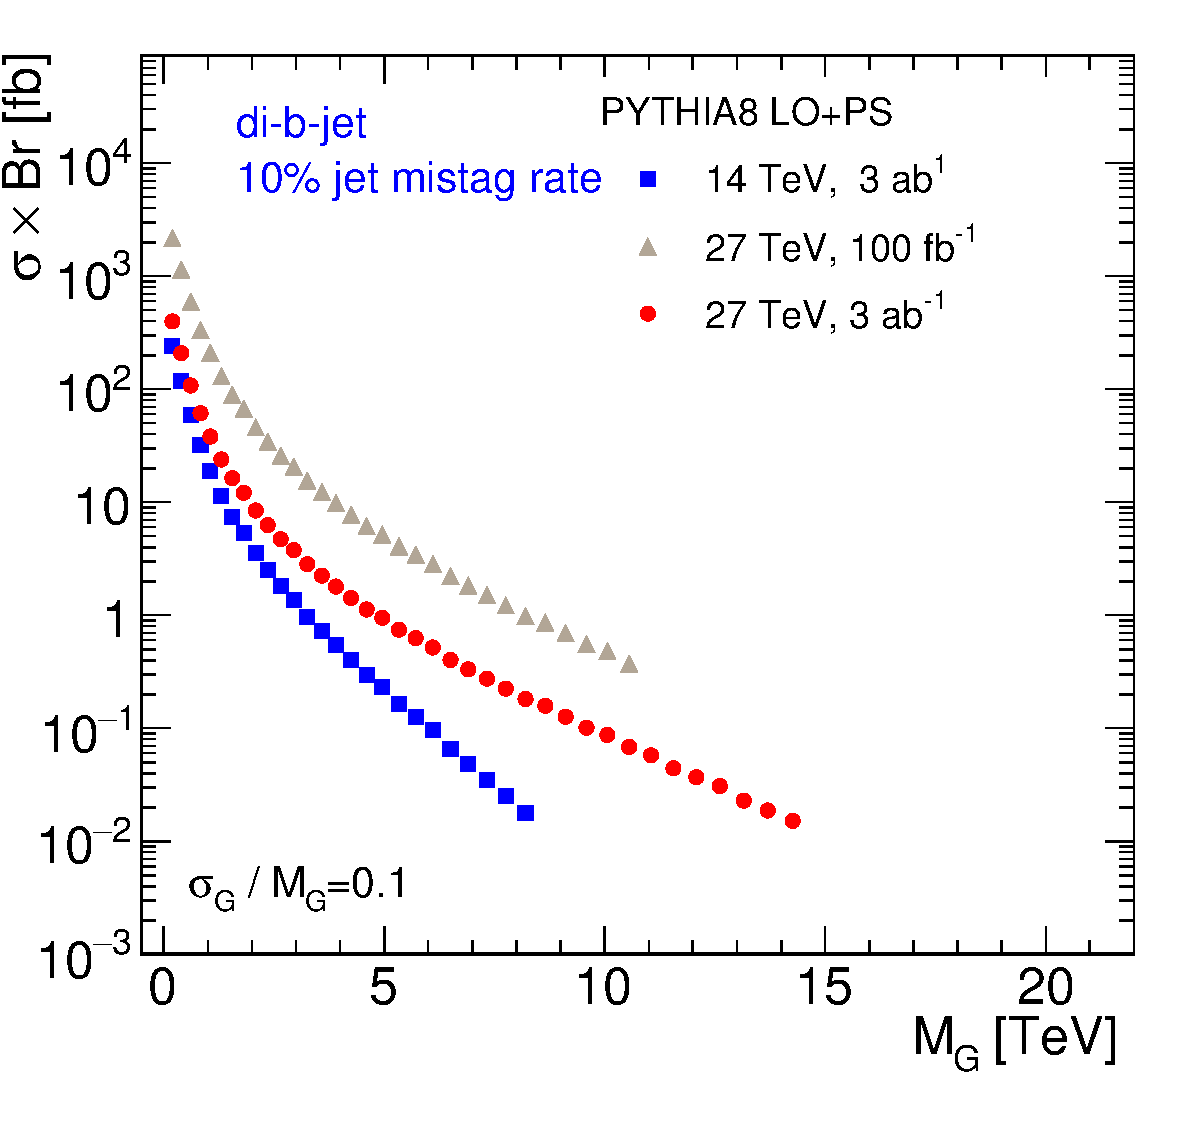
\includegraphics[width=0.7\textwidth]{\main//section7OtherSignatures/img/JetJetMass_2bjet.pdf}
\end{center}
\caption{The 95\%~\cl upper limits obtained from the
$M_{jj}$  distribution for jets identified as $b$-jets.
The limits are set on fiducial cross-section times the  branching ratio to two jets
for a hypothetical BSM signal approximated by a Gaussian contribution to the dijet mass spectrum.  The limits are obtained for the HL-LHC and HE-LHC energies.}
\label{fig:JetJetMass_bjet}
\end{figure}

Figure~\ref{fig:14tev_JetJetMass_2jet} shows two representative 
$M_{jj}$ distributions using the simulations discussed above. The results are shown for the HL-LHC and HE-LHC colliders using different integrated luminosities,  3~ab$^{-1}$ and 100~fb$^{-1}$, respectively. The figure also shows contributions to the total event rate 
from $W/Z/H^0$-boson processes combined  and
top-quark processes from the hard interactions (shown separately).
The lower panel shows the relative statistical uncertainty on the
data points, i.e. $\Delta d_i/d_i$, where $d_i$ is the number of
the events in the bins, and $\Delta d_i$ its statistical uncertainty (which is $\sqrt{d_i}$ in the case of counting statistics). For a quantitative characterization of the dijet mass reach,
the dashed lines on the lower panel show the $M_{jj}$ point at which
statistical uncertainty in a bin is 100\% (or $\Delta d_i/d_i=1$). We have chosen this point 
to define the statistical reach for the measurements using the $M_{jj}$ distributions.
The $M_{jj}$  mass reach at the \com of 27~TeV is close to
$17$~TeV,  even for the modest luminosity of 100~fb$^{-1}$. This is a factor of 1.5
larger than the dijet mass reach for the luminosity expected at the HL-LHC.

\begin{figure}[ht]
\begin{center}
   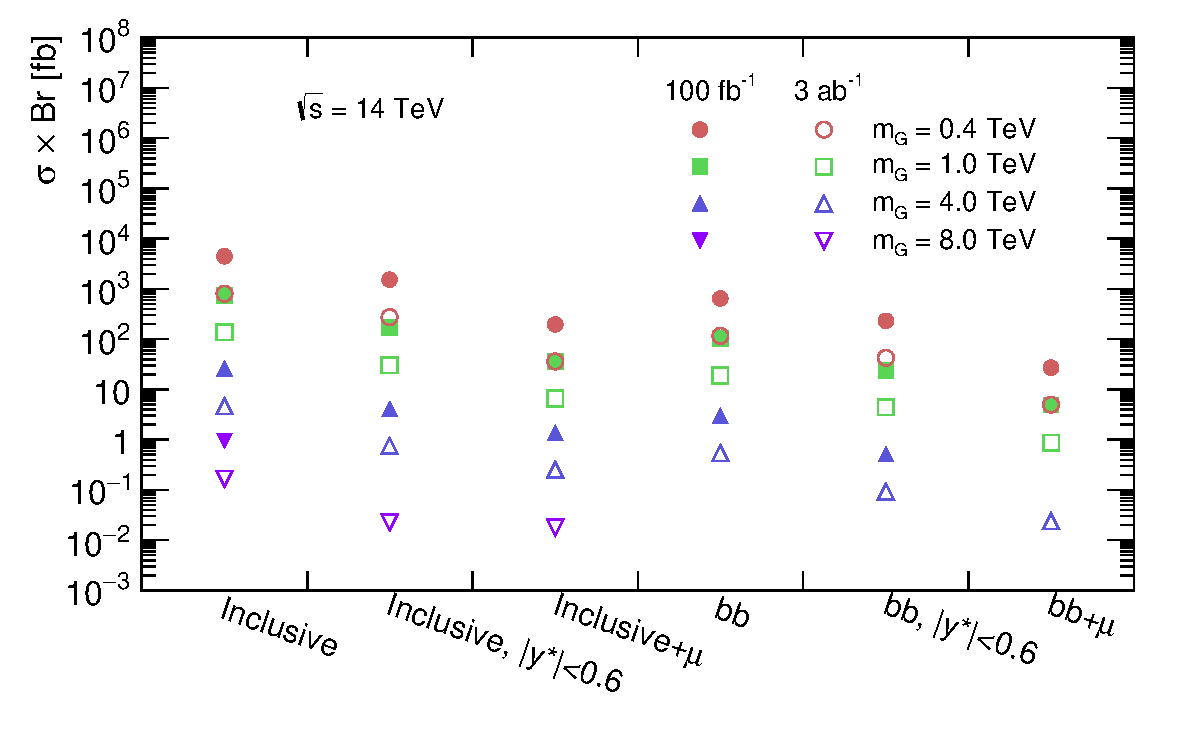
\includegraphics[width=0.8\textwidth]{\main//section7OtherSignatures/img/mass_limit_gauss_comp_14tev.pdf}
   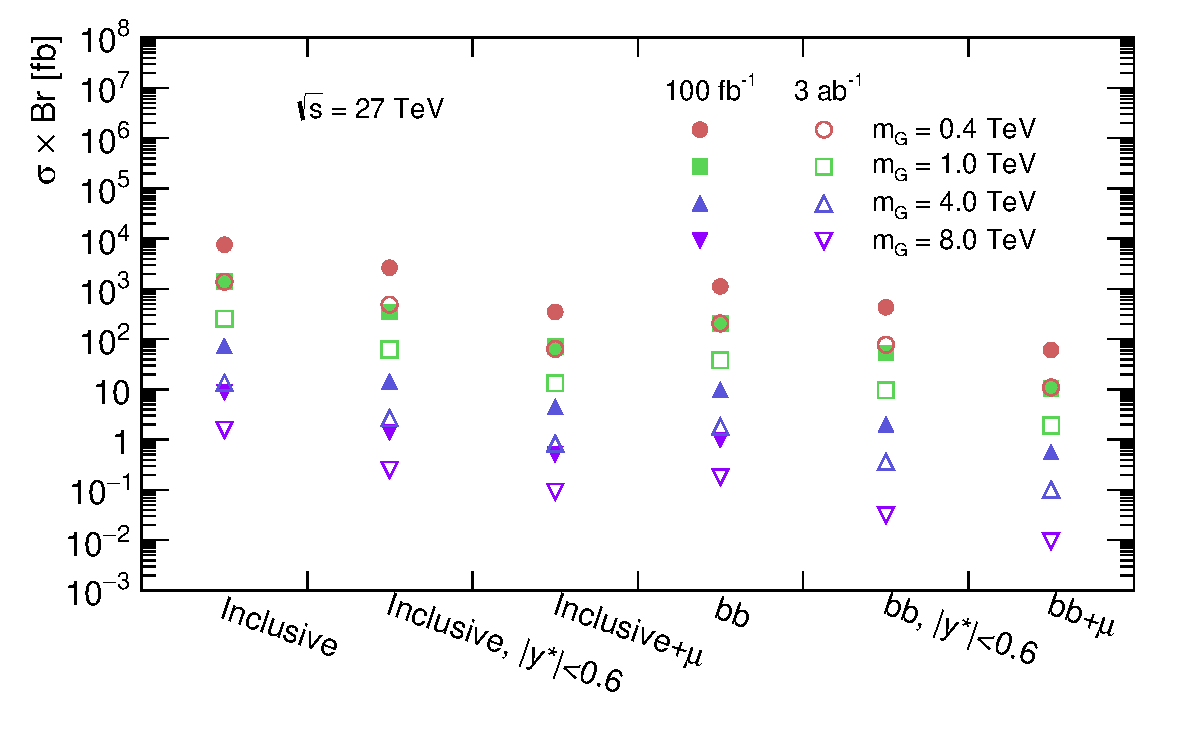
\includegraphics[width=0.8\textwidth]{\main//section7OtherSignatures/img/mass_limit_gauss_comp_27tev.pdf}
\end{center}
\caption{Comparisons of the  95\%~\cl upper limits obtained from the
$M_{jj}$  distribution at 14 TeV (right) and 27 TeV (left). Limits at 0.4~TeV, 1~TeV, 4~TeV and 8~TeV  are shown for 100 fb$^{-1}$ data and 3 ab$^{-1}$ data in different channels with different selections, respectively. }
\label{fig:JetJetMass_comp}
\end{figure}

The dijet distributions discussed above were used to set  the 95\%~\cl 
upper limit on fiducial cross-section times the 
branching ratio for a generic Gaussian signal with
the width ($\sigma_G$) being  10\% of the Gaussian peak position.
Figure~\ref{fig:JetJetMass_jet} shows the  obtained limits.    
In addition to inclusive dijet events, this figure shows the upper limits
for events with at least one isolated muon with transverse momentum above 60~GeV.
The results show that  the HE-LHC experiment with an integrated luminosity of 100 fb$^{-1}$ have advantages
over the HL-LHC in terms of statistical sensitivity to high-mass states. 
When using the same integrated luminosity (3~ab$^{-1}$) for HL-LHC and HE-LHC, 
the HE-LHC provides a factor of two 
larger reach for masses compared to the HL-LHC. The expected limit for 3~ab$^{-1}$ at the HE-LHC 
is a factor of ten better than for 100~fb$^{-1}$ .

Figure~\ref{fig:JetJetMass_bjet} shows the 95\%~\cl upper limits obtained from the $M_{jj}$ distribution for events where both leading jets were identified as $b-$jets.
As for the previous simulation based on inclusive jets, physics reach of the HE-LHC is larger than that of the HL-LHC, assuming 100 fb$^{-1}$ for the HL-LHC project.

Figure~\ref{fig:JetJetMass_comp} shows the comparisons of the limits for dijet and muon associated dijet channels with inclusive  or $b$-tagging selections for the 14~TeV and 27~TeV collision energies. 
In addition to the inclusive jet case, we also calculated the upper limits after applying the rapidity difference requirement $|y^*|<0.6$ between two  jets~\cite{ATLAS:2015nsi}  in order to enhance the sensitivity to heavy
BSM particles decaying to jets.

The studies discussed ~\cite{Chekanov:2017pnx} have also shown that searches for signals in dijets invariant masses require well-understood estimates for the $M_{jj}$ background shape. 
An example of such challenging background shape is shown in \fig{fig:14tev_JetJetMass_2jet}.
A data-driven determination of the shape background at the HL-LHC and  HE-LHC
should be performed with the relative statistical precision
of  $0.01\%$ per data point for $M_{jj}<1$~TeV. 
Currently, it is difficult to achieve 
such precision using the available tools used for the LHC run 2 data.

In conclusion, it was illustrated
that the HE-LHC provides substantial improvements for searches of new physics in dijet invariant masses,  compared to searches  at the HL-LHC.
Even for a rather modest 100~fb$^{-1}$ luminosity of the HE-LHC project, the simulations show that the 
mass reach for dijet searches is about 50\% larger than that from the HL-LHC with 3 ab$^{-1}$.
The reported limits can be used for exclusions of BSM resonances decaying that
decay to form two jets in inclusive dijet events, events with di-$b$-jets, and events with associated muons. Note that the actual exclusion ranges significantly depend on expected  cross-sections and branching ratios of BSM models for the LH-LHC and HE-LHC collision energies.

\section*{Acknowledgments}

The submitted manuscript has been created by UChicago Argonne, LLC,
Operator of Argonne National Laboratory (``Argonne'').
Argonne, a U.S. Department of Energy Office of Science laboratory,
is operated under Contract No. DE-AC02-06CH11357.
This research was made possible by an allocation of computing time through the ASCR Leadership Computing Challenge (ALCC) program. This research used resources of the National Energy Research Scientific Computing Center, a DOE Office of Science User Facility supported by the Office of Science of the U.S. Department of Energy under Contract No. DE-AC02-05CH11231.



